\documentclass{article}
\usepackage{graphicx} % Required for inserting images
\usepackage{float}

\title{\textbf{"Summary of The Role of Women in Modern Artificial Intelligence and Robotics”}}
\author{\textbf{Muhammad Ayyan}\\
\textbf{Roll no:} l260754\\
\textbf{Section :} BCS-1F}
\date{September 2026}


\begin{document}

\maketitle

\tableofcontents
\section{Introduction and contents}

Artificial Intelligence (Ai) is growing rapidly in all over the world and its need of work is also increasing day by day. So everyone is working on it, but women are significantly behind in these kinds of field . This article is motivating the women of the whole world to participate in such kinds of activities.


\section{Current situation}
In recent years, the participation of women in the fields of artificial intelligence (AI) and robotics has become a globally relevant issue. Various scientific articles, international reports, and many other platforms confirm this issue and also propose solutions to it.

\subsection{Key facts and statistics}
\begin{itemize}
    \item \textbf{Workforce \& Research:}
In recent years, almost only 22 \% of the scientific research papers on Ai technology is being published by the woman authors or scientist, which shows the male dominance in this field. Women make up only 26 \% of the global workforce in AI/tech.

\item \textbf{Research Authorship:} Only 11\% of AI research papers are written solely by women, compared to 55\% written only by men 
\begin{figure}{H}
    \centering
    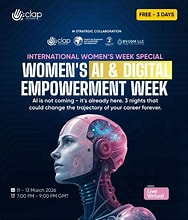
\includegraphics[width=0.5\linewidth]{OIP.jpg}
    \caption{Women Empowerment work}
    \label{fig:placeholder}
\end{figure}

\end{itemize}


\begin{enumerate}
    \item woman in culture always been an essential part of the society
    \item woman in developing society is a part of the society that cannot be neglected
    \dots Woman 
\end{enumerate}

\begin{table}
\centering
    \begin{tabular}{l|r|c}
            \hline\textbf{Initiative Name} &\textbf{Primary Target Group} & \textbf{Key Programs}\\\hline
       Women in AI & Women professionals, researchers, and students & Provides mentorship, technical training, and networking events \\\hline
        Girls Who Code & School and college female students & Offers coding bootcamps, learning grants, and hands-on tech projects \\\hline
         Women in AI & Women professionals, researchers, and students & Provides mentorship, technical training, and networking events \\
        Girls Who Code & School and college female students & Offers coding bootcamps, learning grants, and hands-on tech projects \\\hline
        
    \end{tabular}
    \caption{Caption}
    \label{tab:placeholder}
\end{table}

\subsection{Key Barriers Faced by Women}
\begin{itemize}
    \item \textbf{Social Stereotypes:} Society often views AI and robotics as male fields, which turns girls away from tech \cite{haydarova2025}.
    \item \textbf{Educational Disparities:} Girls get less exposure to advanced math and computer science early on \cite{haydarova2025}.
    \item \textbf{Workplace Inequality:} Women in tech often face unequal pay, fewer promotions, lack of guidance, and workplace discrimination \cite{haydarova2025}.
\end{itemize}

\sectiion{Effective measures}
 Girls need to be engaged in science, mathematics, and computer science from an early age. Introducing advanced technologies during school years and using gender-sensitive curricula helps build confidence and interest. This early exposure is crucial because it shapes positive attitudes toward technology and breaks down stereotypes that these fields are “male-dominated.”

 
\subsection{Strategic Measures for Improvement}
\begin{enumerate}
    \item \textbf{Ensure Gender Equality in Early Education:} Introduce computer science early in school and use gender-friendly study materials 
    \item \textbf{Establish Mentorship Programs:} Connect young women with experienced professionals to help guide their careers.
    \item \textbf{Fund Female-Led Research:} Provide dedicated grants for women researchers and women-led tech startups.
    \item \textbf{Run Public Awareness Campaigns:} Share stories of successful women in tech through media to inspire younger generations.
\end{enumerate}

\section{Conclusion and Significance}
Getting more women into AI and robotics is not just about fairness; it makes technology better for everyone \cite{haydarova2025}. Diverse teams build fairer tools and prevent bias in AI systems \cite{haydarova2025}. Schools, governments, and tech companies need to work together to clear these barriers and make space for women as tech creators \cite{haydarova2025}.

\begin{thebibliography}{99}
\bibitem{haydarova2025}
K. Haydarova, ``The Role of Women in Modern Artificial Intelligence and Robotics,'' \textit{International Journal of Artificial Intelligence}, vol. 5, no. 4, pp. 716--721, 2025.

\bibitem{unesco2021}
UNESCO, \textit{Cracking the code: Girls' and women's education in STEM}, United Nations Educational, Scientific and Cultural Organization, 2021.
\end{thebibliography}

\end{document}
